\mode*

\begin{frame}
  \tableofcontents
\end{frame}

\section{Vad är programmering?}

% Fokus programmering (=vad är programmering), varför läsa programmering, 
% datasäkerhet/kryptering. Bra att få med:

\begin{frame}
  \begin{block}{Vad är programmering?}
    \begin{itemize}
      \item Programmering betyder att skriva program.
      \item Program implementerar algoritmer, exempelvis gör så att datorn kan 
        köra en viss algoritm.
      \item Algoritmer är sätt att göra någonting på.
    \end{itemize}
  \end{block}

  \pause

  \begin{exercise}[Välkända algoritmer]
    \begin{itemize}
      \item Känner ni till några algoritmer?
    \end{itemize}
  \end{exercise}
\end{frame}

\begin{frame}
  \begin{example}[Att göra pannkakssmet]
    \begin{enumerate}
      \item Knäck tre ägg i en bunke.
      \item Vispa ordentligt.
      \item Häll i \SI{3}{\deci\litre} mjölk.
      \item Vispa ordentligt.
      \item För totalt \SI{3}{\deci\litre} mjöl:
        \begin{enumerate}
          \item Häll i \SI{1}{\deci\litre} mjöl.
          \item Vispa ordentligt.
        \end{enumerate}
      \item Häll i \SI{\frac{1}{2}}{tsk} salt.
      \item Häll i \SI{2}{msk} smält smör.
      \item Vispa ordentligt.
    \end{enumerate}
  \end{example}
\end{frame}

\begin{frame}
  \begin{example}[Att steka pannkakor]
    \begin{enumerate}
      \item Gör pannkakssmet.
      \item För varje portion:
        \begin{enumerate}
          \item Häll \SI{1}{\deci\litre} smet i en het stekpanna.
          \item Vänta \SI{2}{\minute}.
          \item Vänd pannkakan.
          \item Vänta \SI{2}{\minute}.
          \item Servera pannkakan.
        \end{enumerate}
    \end{enumerate}
  \end{example}
\end{frame}

\begin{frame}
  \begin{example}[Att multiplicera talen \(a\) och \(b\)]
    \begin{enumerate}
      \item Låt \(m = 0\)
      \item För varje siffra i \(a\), börja bakifrån:
        \begin{enumerate}
          \item Beteckna nuvarande siffra i \(a\) med \(s_a\).
          \item För varje siffra i \(b\), börja bakifrån:
            \begin{enumerate}
              \item Beteckna nuvarande siffra i \(b\) med \(s_b\).
              \item Beräkna \(s_{ab} = s_a\cdot s_b + m\).
              \item Beräkna \(m = s_{ab} / 10\) (heltalsdivision)
              \item Om \(s_{ab} > 9\), låt \(s_{ab} = s_{ab} - 10\).
            \end{enumerate}
        \end{enumerate}
    \end{enumerate}
  \end{example}
\end{frame}

\begin{frame}
  \begin{remark}
    \begin{itemize}
      \item Kokbok: en samling program för köket.
      \item Exekveras i normalfallet av människor.
      \item Men ibland av maskiner i fabriker.
    \end{itemize}
  \end{remark}

  \pause

  \begin{remark}
    \begin{itemize}
      \item Datorprogram implementerar algoritmer som kan exekveras av datorer.
    \end{itemize}
  \end{remark}
\end{frame}


\section[Var finns det?]{Var finns programmering?}

% Var finns programmering?

\begin{frame}
  \begin{example}[Fordon]
    \begin{itemize}
      \item Sitter hundratals datorer i en bil idag.
    \end{itemize}
  \end{example}

  \begin{example}[Ekonomiska system]
    \begin{itemize}
      \item Bankomaterna
      \item Internetbanken
      \item Swish
      \item Terminalerna i butikerna
    \end{itemize}
  \end{example}

  \begin{example}[Kritisk infrastruktur]
    \begin{itemize}
      \item Kraftverk
      \item Industriell produktion
    \end{itemize}
  \end{example}
\end{frame}

\begin{frame}
  \begin{example}[Servrar på webben]
    \begin{itemize}
      \item Varenda webbsida är utmatningen av ett program.
      \item Ibland innehåller själva webbsidan program som webbläsaren kör 
        (Javascript).
    \end{itemize}
  \end{example}
\end{frame}


\section[Vad är det bra för?]{Vad är programmering bra för?}

\begin{frame}
  \begin{question}
    \begin{itemize}
      \item Varför göra något som en dator/robot kan göra bättre?
    \end{itemize}
  \end{question}
\end{frame}

\begin{frame}
  \begin{example}[Hemautomation]
    \begin{itemize}
      \item Robotdammsugare
      \item Robotgolvmoppar
      \item Automatiska lysen (var någon är hemma, om solen gått ned)
      \item Kontroll av energianvändning
    \end{itemize}
  \end{example}
\end{frame}

\begin{frame}
  \begin{example}[Automation i mitt jobb]
    \begin{itemize}
      \item Föra över betyg från lärplattformen till nationella 
        betygsdatabasen.
      \item Samla in statistik för hur det går för studenterna.
    \end{itemize}
  \end{example}

  \begin{example}[Räkna på data]
    \begin{itemize}
      \item Vad är Sveriges vanligast namn?
      \item Får eleverna högre betyg i matematik efter att de lärt sig att 
        programmera?
    \end{itemize}
  \end{example}
\end{frame}

% Ett program kan endast utföra de operationer som tilldelats, det tänker inte 
% själv.

\begin{frame}
  \begin{example}[\enquote{Framtida} automation]
    \begin{itemize}
      \item Självkörande fordon
      \item \enquote{Smarta} städer
    \end{itemize}
  \end{example}

  \pause

  \begin{remark}
    \begin{itemize}
      \item Datorer är inte smartare än vad vi gör dem.
      \item De följer bara instruktioner.
    \end{itemize}
  \end{remark}
\end{frame}


\section[Kan det vara farligt?]{Hur kan programmering vara farligt?}

% Hur kan programmering användas på ett skadligt sätt?

% Programkoden är (i ett normalt interface) osynlig för användaren, användaren 
% vet inte vad programmet gör i bakgrunden.

% Användaren vet inte vilken information som insamlas/används. Exempel: 
% Facebook följer allt du gör på nätet, t.ex. hur du surfar mellan hemsidor och 
% vilka. Detta sker även när du inte är inloggad.

% Många program (s.k. bottar) är framtagna för att bedriva propaganda, påverka 
% val och manipulera resultat/statistik. Dessa program analyserar användaren 
% och tar reda på hur du tänker tycker i dagsläget, för att så effektivt som 
% möjligt påverka dig att tycka och tänka annorlunda.

\begin{frame}
  \begin{figure}
    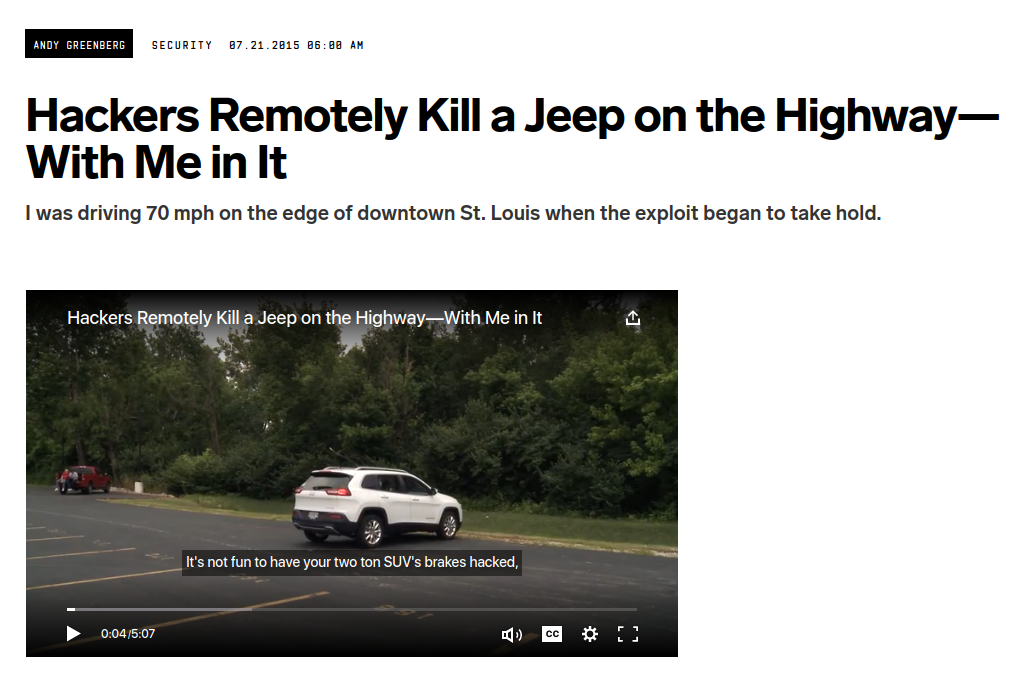
\includegraphics[width=\columnwidth]{fig/hacking-jeep.png}
  \end{figure}
\end{frame}

\begin{frame}
  \begin{example}[Spårning på webben]
    \begin{itemize}
      \item \url{https://clickclickclick.click}
      \item \url{https://amiunique.org/}
      \item \url{https://coveryourtracks.eff.org/}
    \end{itemize}
  \end{example}
\end{frame}

\begin{frame}
  \begin{question}
    \begin{itemize}
      \item Fine, de kan spåra mig på webben.
      \item Varför bry sig?
    \end{itemize}
  \end{question}
\end{frame}

\begin{frame}
  \begin{figure}
    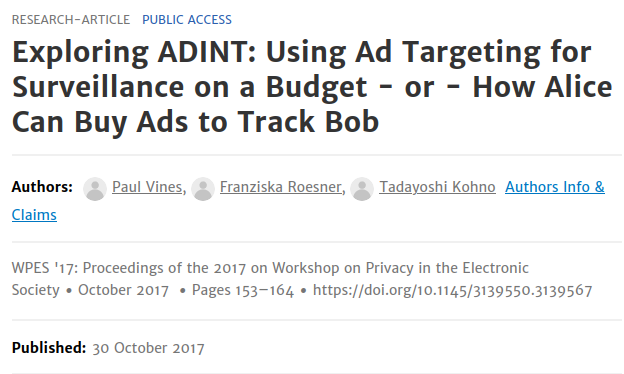
\includegraphics[width=\columnwidth]{fig/adint.png}
  \end{figure}
\end{frame}

\begin{frame}
  \begin{figure}
    
\includegraphics[width=\columnwidth]{fig/listening-assistants.png}
  \end{figure}
\end{frame}

\begin{frame}
  \begin{figure}
    
\includegraphics[height=0.8\textheight]{fig/The-Age-of-Surveillance-Capitalism.jpg}
  \end{figure}
\end{frame}

\begin{frame}
  \begin{figure}
    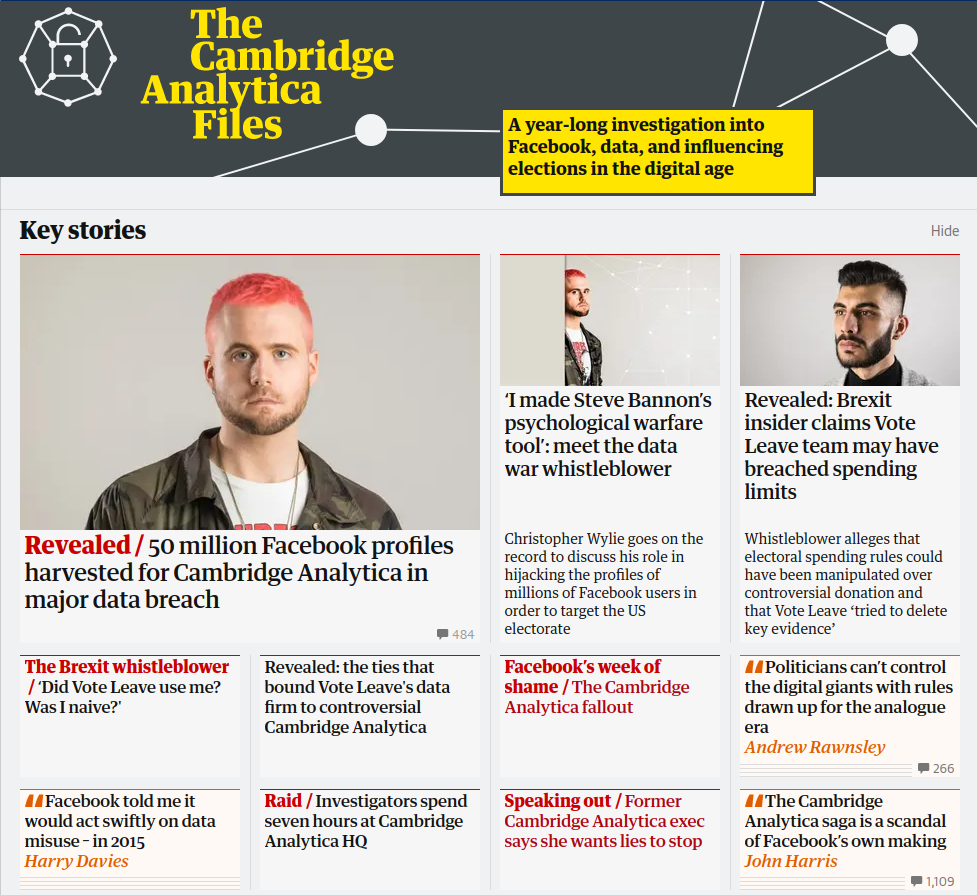
\includegraphics[width=\columnwidth]{fig/analytica.png}
  \end{figure}
\end{frame}

\begin{frame}
  \begin{figure}
    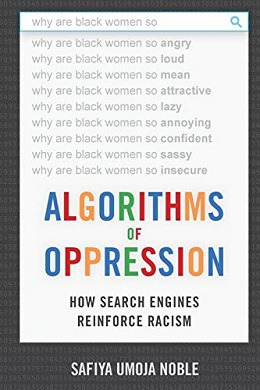
\includegraphics[height=0.8\textheight]{fig/Algorithms-of-Oppression.jpg}
    \only<2>{%
      
\includegraphics[width=0.6\columnwidth]{fig/teens.png}
    }
  \end{figure}
\end{frame}

\begin{frame}
  \begin{figure}
    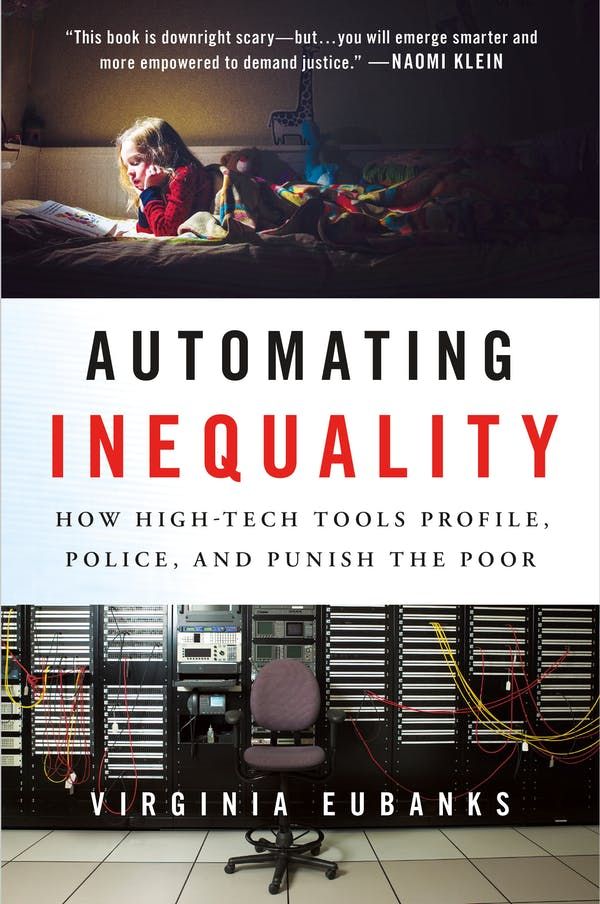
\includegraphics[height=0.8\textheight]{fig/Automating-Inequality.jpg}
    \hspace{2em}
    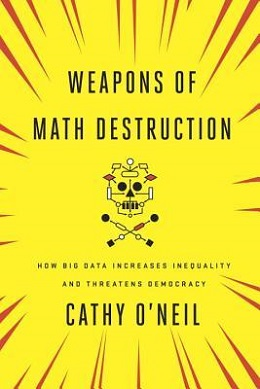
\includegraphics[height=0.8\textheight]{fig/Weapons-of-Math-Destruction.jpg}
  \end{figure}
\end{frame}

\begin{frame}
  \begin{question}
    \begin{itemize}
      \item Hur många var det som tänkte på att alla dessa böcker var skrivna 
        av kvinnor?
    \end{itemize}
  \end{question}
\end{frame}

%\begin{frame}
%  \begin{remark}
%    \begin{itemize}
%      \item Finns massor med problem med saker som automatiserad 
%        beslutsfattning.
%      \item Rekommendationsalgoritmer skapar filterbubblor.
%      \item Och mycket mer.
%    \end{itemize}
%  \end{remark}
%\end{frame}

% Många appar innehåller malware (sabotageprogram) som t.ex. stjäl användarens 
% bilder för att skicka/sälja vidare till tredje part eller ''lyssnar'' på vad 
% du säger genom mikrofonen, även när du är inaktiv.

% Våra samhällssystem bygger på kod och har svagheter (särskilt när någon går 
% in med avsikt att skada system eller läcka information) och därmed föreligger 
% förstås både mindre och större risker, från att mailkonton hackas till att 
% elnät släcks ned.

% Alla system måste byggas med rigida skydd mot sabotage.
% Förhoppningsvis ska detta inte avskräcka utan intressera för vad som
% är och kommer att fortsätta vara ett enormt utvecklingsområde.
% Lektion 8 handlar om arbetsmöjligheter inom data, informationsteknologi (IT), 
% programmering osv. Där kryptering (omkodning av data för att t.ex. skydda 
% lösenord och öka vår personliga säkerhet online) är ett enormt och växande 
% område.

% Dina tankar om GDPR: tillräcklig förordning? Gäller för EU:s
% medborgare, men även amerikanska företeg( tex facebook) måste väl
% tillse att det följs för europeiska användare? Har USA motsvarande
% (bättre/sämre) personuppgiftslag\ldots{}?

% En tanke jag har är att eleverna tror att GDPR skyddar dem\ldots{} men
% så fort de klickar ``godkänn cookies'' så har dom delgivit till saker
% som dom inte har en aning om\ldots{} Inte ens jag vet vad man godkänner,
% ändå klickar man ``godkänn alla'' typ överallt för att komma
% vidare\ldots{} Vad ger man då bort liksom\ldots{}? Det är dom nyfikna
% på.

%\begin{frame}
%  \begin{figure}
%    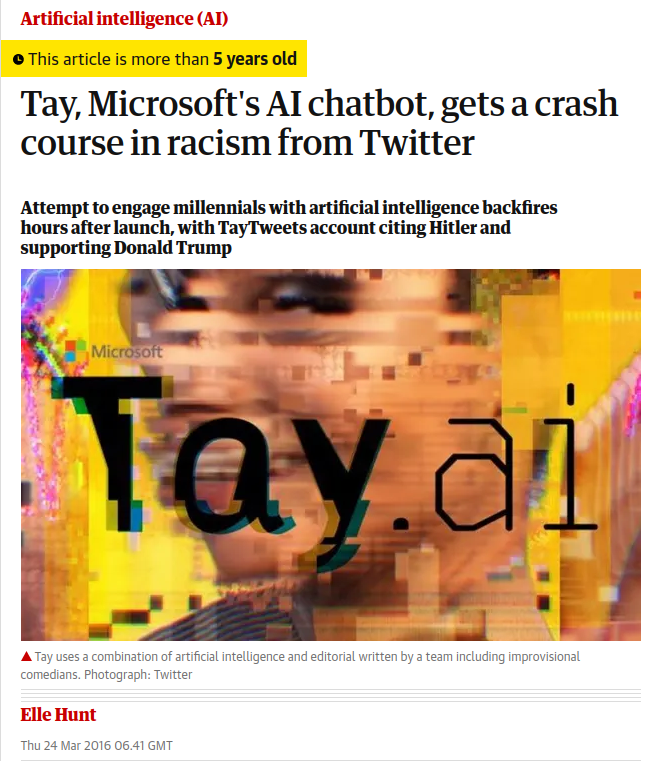
\includegraphics[height=\textheight]{fig/tay.ai.png}
%  \end{figure}
%\end{frame}

% Varför kul/bra att utbilda sig inom och jobba med programmering? (mycket 
% samarbete kanske... bra lön, ökande efterfrågan på kompetens på området)

\section[Framtid inom det?]{En framtid inom programmering?}

\begin{frame}
  \begin{example}[Förståelse]
    \begin{itemize}
      \item Nästintill allt är programmerat.
      \item Man behöver ha en förståelse för programmering för att förstå 
        världen.
    \end{itemize}
  \end{example}

  \begin{example}[Arbete]
    \begin{itemize}
      \item Fler arbeten kommer att kunna automatiseras med programmering.
      \item Kommer att behövas många fler som kan programmera.
    \end{itemize}
  \end{example}
\end{frame}

